\documentclass[12pt,a4paper,oneside]{article}
\usepackage[utf8]{inputenc}
\usepackage{amsmath}
\usepackage{algorithm}
\usepackage{algpseudocode}
\usepackage{varwidth}
\usepackage{graphicx}

\makeatletter
\def\BState{\State\hskip-\ALG@thistlm}
\let\OldStatex\Statex
\renewcommand{\Statex}[1][3]{%
\setlength\@tempdima{\algorithmicindent}%
\OldStatex\hskip\dimexpr#1\@tempdima\relax}
\makeatother
\let\oldReturn\Return
\renewcommand{\Return}{\State\oldReturn}
\providecommand{\abs}[1]{\lvert#1\rvert}

\date{}

\author{Gabriel Rodríguez Canal}
\title{Seam Carving - Algoritmos y Computación}

\begin{document}

\maketitle

\section{Introducción}

Seam Carving es un algoritmo de reescalado de imágenes con conocimiento del contenido.
A diferencia del reescalado clásico, es capaz de modificar el tamaño de la imagen sin
perturbar los elementos más significativos de la imagen (el algoritmo determina qué
elementos son significativos en función de la energía de la imagen. Estos conceptos se
explican en la sección \ref{fund}).

\section{Fundamentos del algoritmo\label{fund}}
El algoritmo Seam Carving se basa en la eliminación de hilos (del inglés
\textit{seams}) de la imagen. En este documento se trabajará en todo momento con una
imagen de dimensiones nxm. Un hilo vertical se define como:
\begin{equation}
    s^x = \{s_i^x\}_{i=1}^n = \{(x(i),i)\}_{i=1}^n, s.a.  \forall i, \abs{x(i)-x(i-1)} \leq 1
    \label{hseam}
\end{equation}

O lo que es lo mismo, una ruta de píxeles 8-conectada. En el caso de los hilos verticales
la definición es:
\begin{equation}
    s^y = \{s_j^y\}_{j=1}^m = \{(j)\}_{j=1}^n, s.a.  \forall j, \abs{y(j)-y(j-1)} \leq 1
    \label{vseam}
\end{equation}

Para entender el cálculo de los hilos es necesario introducir el concepto de energía de
una imagen.

\subsection{Energía de una imagen}
La energía de una imagen se define como:
\begin{equation}
    e_1(\textbf{I}) = \abs{\frac{\partial}{\partial x} \textbf{I}} + \abs{\frac{\partial}{\partial y} \textbf{I}}
\end{equation}

Las imágenes digitales son discretas, pese a la ilusión conseguida mediante los monitores
de alta resolución. No es posible calcular directamente el gradiente de la imagen. sin
embargo, existen unas aproximaciones numéricas llamadas \textit{kernels} basados en la
convolución matemática discreta que permiten calcular el gradiente para cada pixel de la
imagen. La energía es, por tanto, una medida de la importancia de cada píxel en la imagen.

Existen numerosos \textit{kernels} orientados al tratamiento de imagenes. Para el presente
trabajo se ha escogido el operador de Sobel por ofrecer buenos resultados en la mayoría de
las imagenes (en ocasiones es conveniente el uso de otros \textit{kernels} más específicos
para algunos tipos de imagenes, con objeto de evitar artefactos y conseguir resultados
más realistas para el ojo humano. La consideración de otros \textit{kernels} escapa al 
propósito de este trabajo).

\subsection{Problema a resolver}
Dada una función de energía \textit{e} el coste o energía de un hilo se define como:
\begin{equation}
    E(\textbf{s}) = E(\textbf{I}_\textbf{s}) = \sum_{i=1}^n e(\textbf{I}(s_i))
\end{equation}

El problema de Seam Carving consiste en minimizar la energía total de dicho hilo, i.e.:
\begin{equation}
    s^* = \min_s \sum_{i=1}^n e(\textbf{I}(s_i))
    \label{problem}
\end{equation}

De este modo se elimina el hilo que contiene menos información de la imagen, manteniéndose
inalterados los elementos que el ojo humano percibe como relevantes.

\section{Solución: programación dinámica}
El problema planteado en la ecuación \ref{problem} admite una traducción sencilla a programación 
dinámica:
\begin{equation}
    M(i,j) = e(i,j) + \min (M(i-1, j-1), M(i-1,j), M(i-1, j+1))
\end{equation}

Para obtener el hilo de mínima energía basta con hacer \textit{backtracking} buscando el 
píxel con menor valor en la última fila de M (o columna si se busca un hilo horizontal)
en el primer paso y ascender hasta la primera fila del mapa M, buscando siempre el vecino
de la fila correspondiente con menor valor en el mapa.

\section{Algoritmo y análisis de coste}
\subsection{Algoritmo básico - reducción de tamaño}
En esta sección se proporciona el pseudocódigo de las funciones principales que componen
el algoritmo de Seam Carving. Para cada una de ellas se ha diseñado una tabla que muestra
el coste de cada línea (aquellas que lo tengan) y el número de veces que se ejecuta. En
general se muestra el número medio de veces que se ejecuta la línea, excepto en la tabla
\ref{fixLSeamTable}, en la que se dan tanto el número de ejecuciones en el peor caso (W)
como en el caso promedio (A). Aunque el estudio se realiza para hilos verticales es
equivalente para hilos horizontales, dado que para el cálculo de estos últimos se utilizan
las mismas funciones con la matriz original de la imagen traspuesta.

\begin{algorithm}
    \caption{Cálculo del hilo}\label{getSeam}
    \begin{algorithmic}[1]
        \Function{getSeam}{$imgray, e$}
        \State Sea $M[1 \ldots {n}, 1 \ldots m] $ un nuevo array
        \State $M[1] = e[1]$   \Comment{Inicialización del mapa de energía}
        \For {$ i = 2 $ to ${n}$}
            \For {$ j = 1 $ to ${m}$}
                \State $M[i, j] = e[i, j] + \min (M[i-1, j-1:j+2])$
            \EndFor
        \EndFor

        \Comment {Backtracking}

        \State Sea $seam[1 \ldots n]$ un nuevo array \Comment se está suponiendo hilo horizontal
        \State $seam[n] = \min (M[n])$
        \For {$i = {n-1}$ to 1}
            \State $seam[i] = seam[i+1] + \min (M[i, seam[i-1]-1:seam[i-1]+2])$
        \EndFor

        \Return $seam$
        \EndFunction
    \end{algorithmic}
\end{algorithm}

\begin{table}
    \center
    \begin{tabular}{|c|c|c|}
        \hline
        línea & coste & nº veces \\
        \hline
        2 & $\mathcal{O}(1)$ & 1 \\
        \hline
        3 & $\mathcal{O}(1)$ & 1 \\
        \hline
        6 & $\mathcal{O}(1)$ & $(n-1) \times m$ \\
        \hline
        9 & $\mathcal{O}(1)$ & 1 \\
        \hline
        10 & $\mathcal{O}(\log{}n)$ & 1 \\
        \hline
        12 & $\mathcal{O}(1)$ & $n-1$ \\
        \hline
    \end{tabular}
    \caption{Análisis del algoritmo \ref{getSeam}}\label{getSeamTable}
\end{table}

La fila 6 de la tabla \ref{getSeamTable} muestra el mayor coste de las operaciones del
algoritmo \ref{getSeam}. De forma asintótica el coste de la función es, por tanto,
 $\mathcal{O}(n \cdot m)$.

\begin{algorithm}
    \caption{Reubicar coordenadas reducción}\label{fixLSeam}
    \begin{algorithmic}[1]
        \Function{fixLastSeam}{$seams$}
            \State $nSeams \gets lenght(seams)$
            \State $previousSeams = seams[1 \ldots nSeams-1]$
            \State $lastSeam = seams[nSeams]$

            \For {$fila = 1$ to n}  \Comment Se supone hilo vertical
                \State $menores \gets 0$
                \For {$s = 1$ to nSeams}
                    \If {$seams[s, fila] < lastSeam[fila]$}
                        \State $menores \gets menores + 1$
                    \EndIf
                \EndFor
                \State $lastSeam[fila] \gets lastSeam[fila] + menores$ 
            \EndFor
        \EndFunction
    \end{algorithmic}
\end{algorithm}

\begin{table}
    \center
    \begin{tabular}{|c|c|c|c|}
        \hline
        línea & coste & nº veces (W)& nº veces(A)\\
        \hline
        2 & $\mathcal{O}(1)$ & 1 & 1\\
        \hline
        3 & $\mathcal{O}(1)$ & 1 & 1\\
        \hline
        4 & $\mathcal{O}(1)$ & 1 & 1\\
        \hline
        6 & $\mathcal{O}(1)$ & n & n\\
        \hline
        8 & $\mathcal{O}(1)$ & $n \times nSeams$ & $n \times nSeams$ \\
        \hline
        9 & $\mathcal{O}(1)$ & $n \times nSeams$ & $n$ \\
        \hline
        12 & $\mathcal{O}(1)$ & $n$ & $n$ \\
        \hline
    \end{tabular}
    \caption{Análisis del algoritmo \ref{fixLSeam}}\label{fixLSeamTable}
\end{table}

$\newline$La fila 8 de la tabla \ref{fixLSeamTable} muestra el mayor coste de las operaciones del
algoritmo \ref{fixLSeam}. De forma asintótica el coste de la función, por tanto,
$\mathcal{O}(n \cdot nSeams)$.

\begin{algorithm}
    \caption{Seam Carving Reducción}\label{seamCarvingR}
    \begin{algorithmic}[1]
        \Function{SeamCarvR}{$imRGB, nSeams$}
            \State Sea $seams[1 \ldots nSeams, 1 \ldots n]$ nuevo array
            \For{$i \gets 1$ to nSeams} 
                \State $imgray \gets rgb2gray(imRGB)$
                \State $e \gets sobel(imgray)$
                \State $seams[i] \gets getSeam(imgray, e)$
                \State $removeSeam(imRGB, seams[i])$
                \State $fixLastSeam(seams)$
            \EndFor
            \Return{$seams$}
        \EndFunction
    \end{algorithmic}
\end{algorithm}

$\newline$A continuación se muestra el operador de Sobel, del que se hará un somero análisis de
 coste para integrarlo en el correspondiente al algoritmo \ref{seamCarvingR}.
\begin{figure}
    \includegraphics[width = \textwidth]{sobelop.png}
\end{figure}

Siendo \textbf{A} la matriz de la imagen y \textbf{*} el operador de convolución: por cada
 píxel han de hacerse 9 productos y 9 sumas para obtener $G_x$. Para una imagen de dimensión
 $n \cdot m$ han de hacerse 18·m·n operaciones; en notación asíntotica, $\mathcal{O}(n \cdot m)$.
 Análogamente, han de hacerse el mismo número de operaciones para obtener $G_y$.
Para obtener G ha de hallarse la potencia 2 de $G_x$ y $G_y$ elemento a elemento. Esto supone
 un coste de $\mathcal{O}(n \cdot m)$ en ambos casos. Para la suma de estas dos matrices se tiene, 
 trivialmente, un coste de $\mathcal{O}(n \cdot m)$ y, finalmente, para la raíz (elemento a elemento),
 se vuelve a tener un coste de $\mathcal{O}(n \cdot m)$. El máximo de todos los costes es
 $\mathcal{O}(n \cdot m)$, coste del operador de Sobel.

$\newline$El coste de la línea 4 será de $\mathcal{O}(n \cdot m)$ en cada iteración, pues se 
trata de una transformación lineal del valor de cada píxel.

\begin{table}
    \center
    \begin{tabular}{|c|c|c|}
        \hline
        línea & coste & nº veces \\
        \hline
        1 & $\mathcal{O}(1)$ & 1 \\
        \hline
        4 &  $\mathcal{O}(n \cdot m)$ & nSeams \\
        \hline
        5 & $\mathcal{O}(n \cdot m)$ & nSeams \\
        \hline
        6 & $\mathcal{O}(n \cdot m)$ & nSeams \\
        \hline
        7 & $\mathcal{O}(n)$ & nSeams \\
        \hline
        8 & $\mathcal{O}(nSeams \cdot n)$ & nSeams \\
        \hline
    \end{tabular}
    \caption{Análisis del algoritmo \ref{seamCarvingR}}\label{seamCarvingRTable}
\end{table}

$\newline$La fila 6 de la tabla \ref{seamCarvingRTable} muestra el mayor coste de las operaciones del
algoritmo \ref{seamCarvingR}, es decir, el algoritmo en estudio, Seam Carving. \textbf{De forma asintótica 
el coste del algoritmo es, por tanto, $\mathcal{O}(nSeams \cdot n \cdot m)$.}

\subsection{Bonus - ampliación de tamaño}
\begin{algorithm}
    \caption{Reubicar coordenadas ampliación}\label{fixNSeam}
    \begin{algorithmic}[1]
        \Function{fixNSeam}{$currSeamInd, seams$}
            \State $currSeam \gets seams[currSeamInd]$
            \State $otherSeams \gets seams[-currSeamInd]$    \Comment Se elimina currSeam

            \For{$fila \gets 1$ to $n$}
                \For{$s \gets 1$ to $length(otherSeams)$}
                    \If{$otherSeams[s, fila] > currSeam[fila]$}
                        \State{$otherSeams[s, fila] \gets otherSeams[s, fila] + 1$}
                    \EndIf
                \EndFor
            \EndFor
        \EndFunction
    \end{algorithmic}
\end{algorithm}

\begin{table}
    \begin{tabular}{|c|c|c|c|}
        \hline
        línea & coste & nº veces (W) & nº veces (A) \\
        \hline
        2 & $\mathcal{O}(1)$ & 1 & 1 \\
        \hline
        3 & $\mathcal{O}(1)$ & 1 & 1 \\
        \hline
        6 & $\mathcal{O}(1)$ & $n \times lenght(otherSeams)$ & $n \times length(otherSeams)$ \\
        \hline
        7 & $\mathcal{O}(1)$ & $n \times length(otherSeams)$ & $n$ \\
        \hline
    \end{tabular}
    \caption{Análisis del algoritmo \ref{fixNSeam}}\label{fixNSeamTable}
\end{table}

$\newline$La fila 6 de la tabla \ref{fixNSeamTable} muestra el mayor coste de las operaciones del
algoritmo \ref{fixNSeam}, es decir, el algoritmo en estudio, Seam Carving. De forma asintótica 
el coste del algoritmo es, por tanto, $\mathcal{O}(n \cdot length(otherSeams))$. Siguiendo con
la nomenclatura utilizada hasta ahora se puede considerar que $length(otherSeams)$ es 
$nSeams$, de modo que la complejidad (para que la comparación sea más sencilla) se expresa como: 
$\mathcal{O}(n \cdot nSeams)$.


\begin{algorithm}
    \caption{Seam Carving Ampliación}\label{seamCarvingA}
    \begin{algorithmic}[1]
        \Function{SeamCarvA}{imRGB, nSeams}
            \State $seams \gets seamCarvR(imRGB, nSeams)$
            \For{$i \gets 1$ to $nSeams$}
                \State addSeam(imRGB, seams)
                \State fixNextSeam(i, seams)
            \EndFor
        \EndFunction
    \end{algorithmic}
\end{algorithm}

\begin{table}
    \center
    \begin{tabular}{|c|c|c|}
        \hline
        línea & coste & nº veces \\
        \hline
        2 & $\mathcal{O}(nSeams \cdot n \cdot m)$ & 1 \\
        \hline
        4 & $\mathcal{O}(n)$ & nSeams \\
        \hline
        5 & $\mathcal{O}(nSeams \cdot n)$ & nSeams \\
        \hline
    \end{tabular}
    \caption{Análisis del algoritmo \ref{seamCarvingA}}\label{seamCarvingATable}
\end{table}

$\newline$La fila 2 de la tabla \ref{seamCarvingATable} muestra el mayor coste de las operaciones del
algoritmo \ref{seamCarvingA}, es decir, el algoritmo en estudio, Seam Carving. De forma asintótica 
el coste del algoritmo es, por tanto, $\mathcal{O}(nSeams \cdot n \cdot m)$.

\section{Apéndice: resultados}
\subsection{Reducción con hilos verticales}
A continuación se muestra el resultado de aplicar reducción por Seam Carving con 500 hilos:
\begin{figure}[!htb]
    \minipage{0.32\textwidth}
      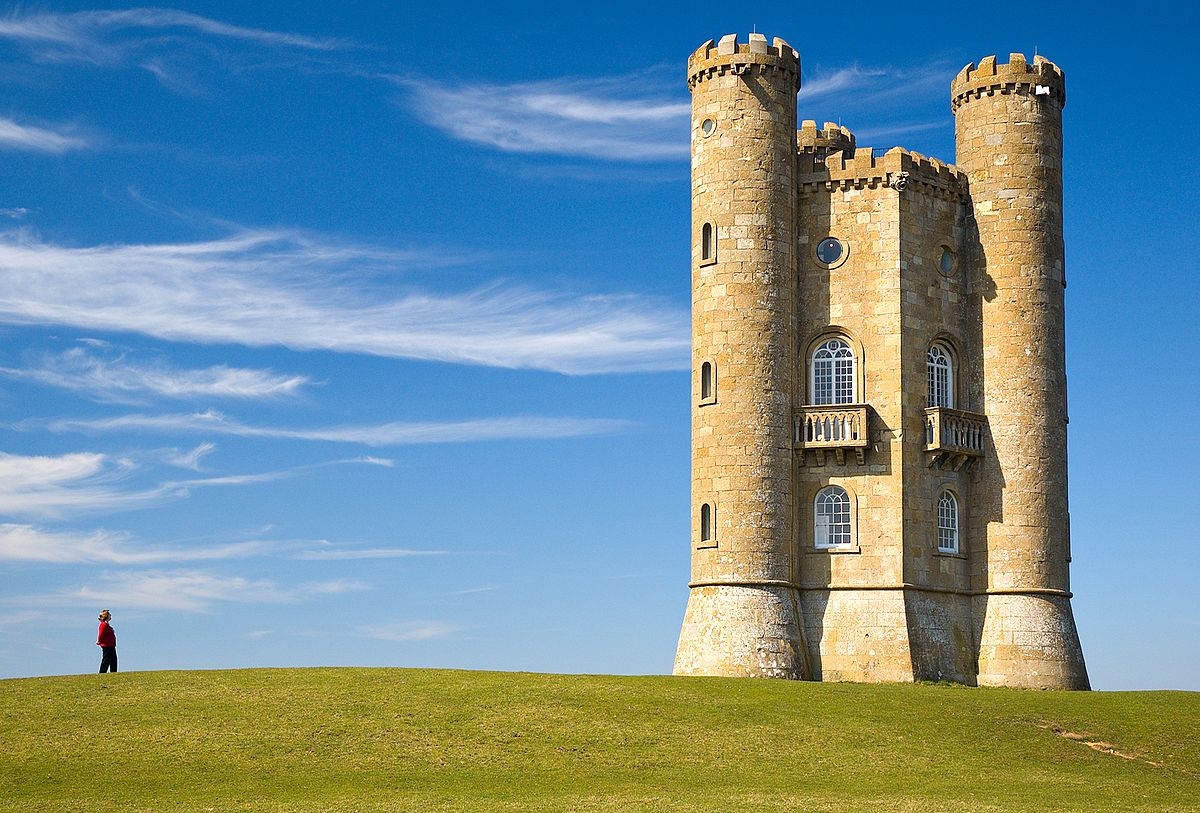
\includegraphics[width=\linewidth]{Broadway_tower_edit.jpg}
      \caption{Imagen original}\label{broadwayorig}
    \endminipage\hfill
    \minipage{0.32\textwidth}
      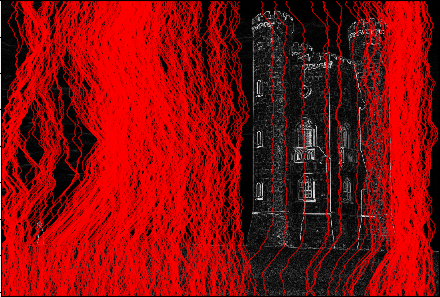
\includegraphics[width=\linewidth]{500-reductionenergy.png}
      \caption{Mapa de energía con 500 hilos superpuestos}\label{broadwayenergy}
    \endminipage\hfill
    \minipage{0.32\textwidth}%
      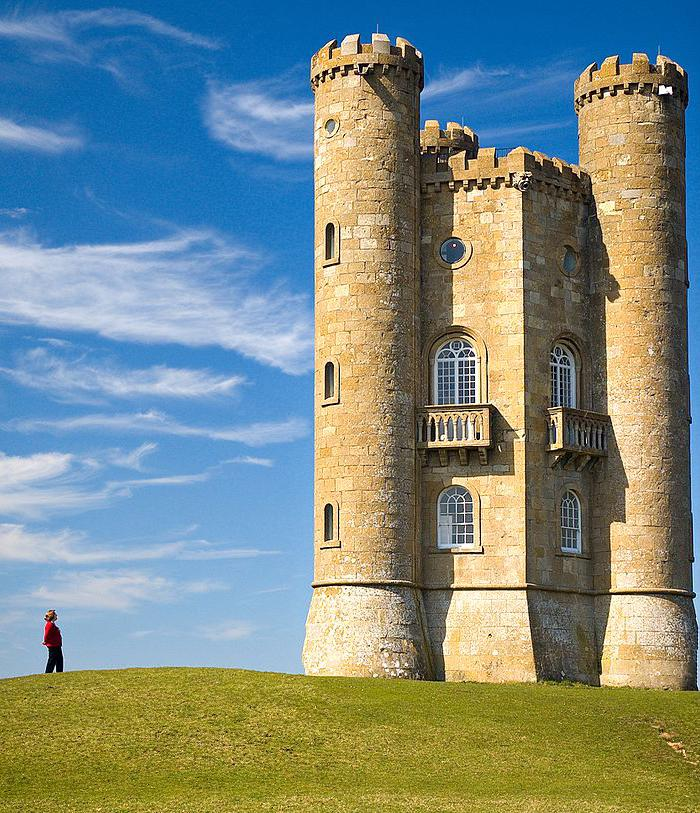
\includegraphics[width=\linewidth]{500-reduction.jpg}
      \caption{Resultado de seam-carving con 500 hilos}\label{broadwayseam}
    \endminipage
\end{figure}

\subsection{Reducción con hilos horizontales}
En las siguientes se imágenes se puede ver el resultado de aplicar reducción por 
Seam Carving vertical con 200 hilos:

\begin{figure}[!htb]
    \minipage{0.32\textwidth}
      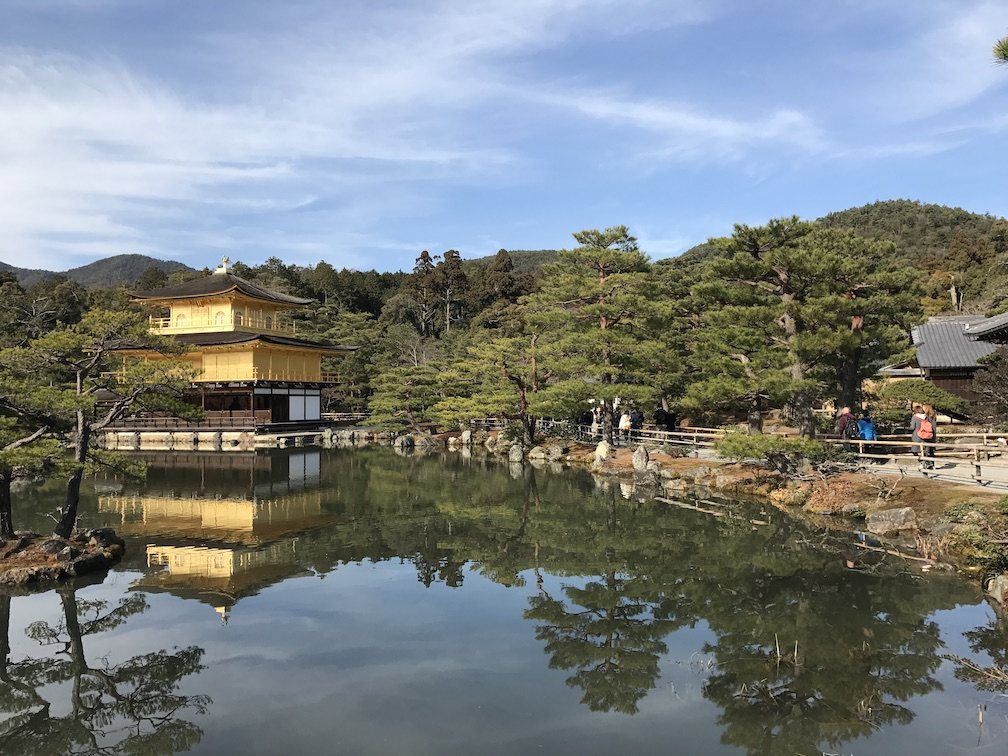
\includegraphics[width=\linewidth]{kinkakuji.jpg}
      \caption{Imagen original}\label{kinkakujiorig}
    \endminipage\hfill
    \minipage{0.32\textwidth}
      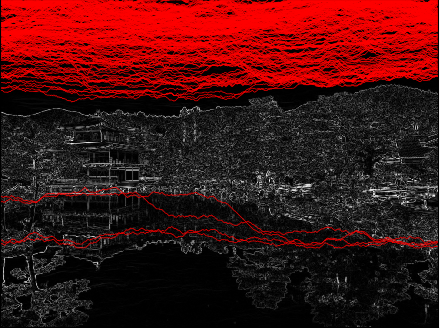
\includegraphics[width=\linewidth]{200-reductionenergyhorizontal.png}
      \caption{Mapa de energía con 200 hilos superpuestos}\label{kinkakujienergy}
    \endminipage\hfill
    \minipage{0.32\textwidth}%
      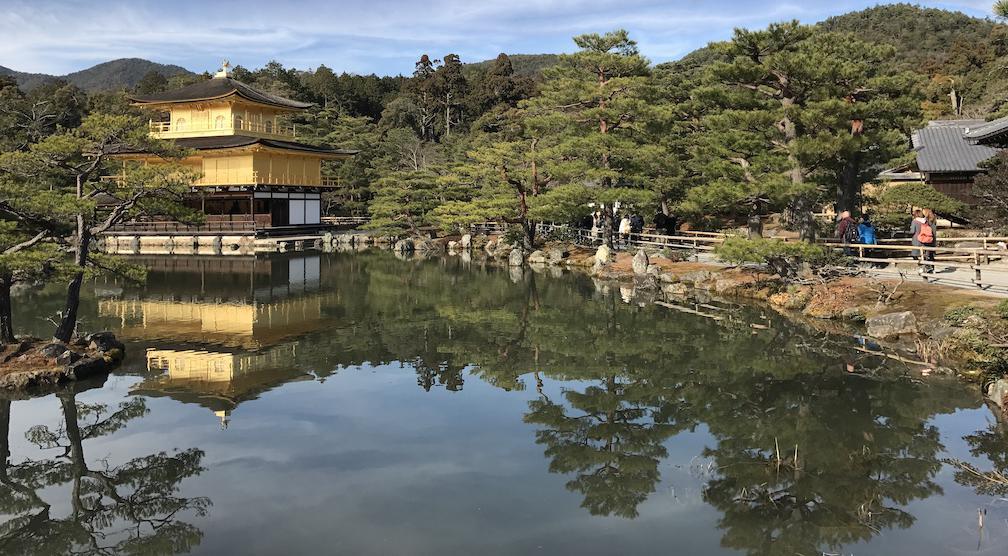
\includegraphics[width=\linewidth]{200-reductionhorizontal.jpg}
      \caption{Resultado de reducción por seam-carving con 200 hilos}\label{kinkakujiseam}
    \endminipage
\end{figure}

\subsection{Ampliación con hilos verticales}
Las siguientes imágenes muestran la ampliación por Seam Carving con 250 hilos verticales:
\begin{figure}[!htb]
    \minipage{0.32\textwidth}
      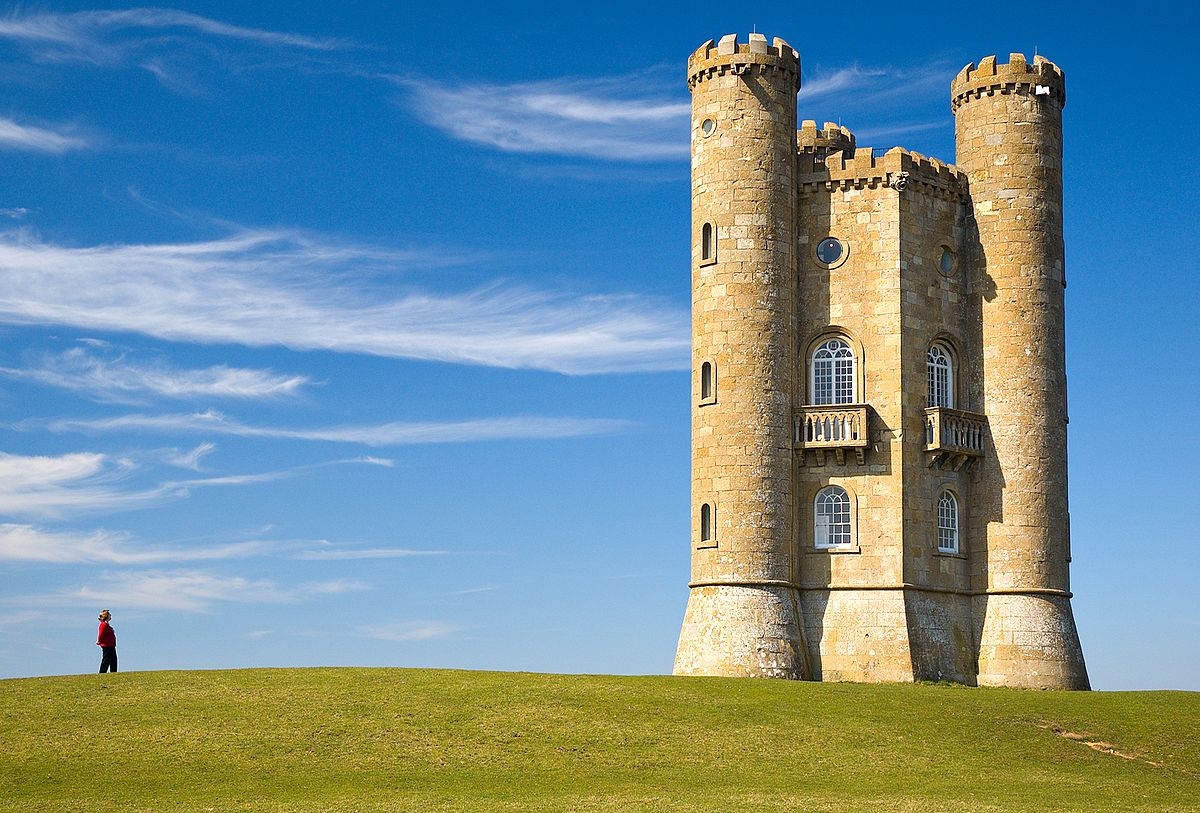
\includegraphics[width=\linewidth]{Broadway_tower_edit.jpg}
      \caption{Imagen original}\label{kinkakujiorig}
    \endminipage\hfill
    \minipage{0.32\textwidth}
      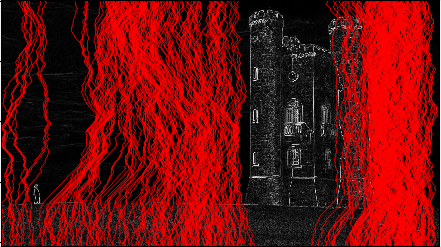
\includegraphics[width=\linewidth]{250-enlargementenergyv.png}
      \caption{Mapa de energía con 250 hilos superpuestos}\label{kinkakujienergy}
    \endminipage\hfill
    \minipage{0.32\textwidth}%
      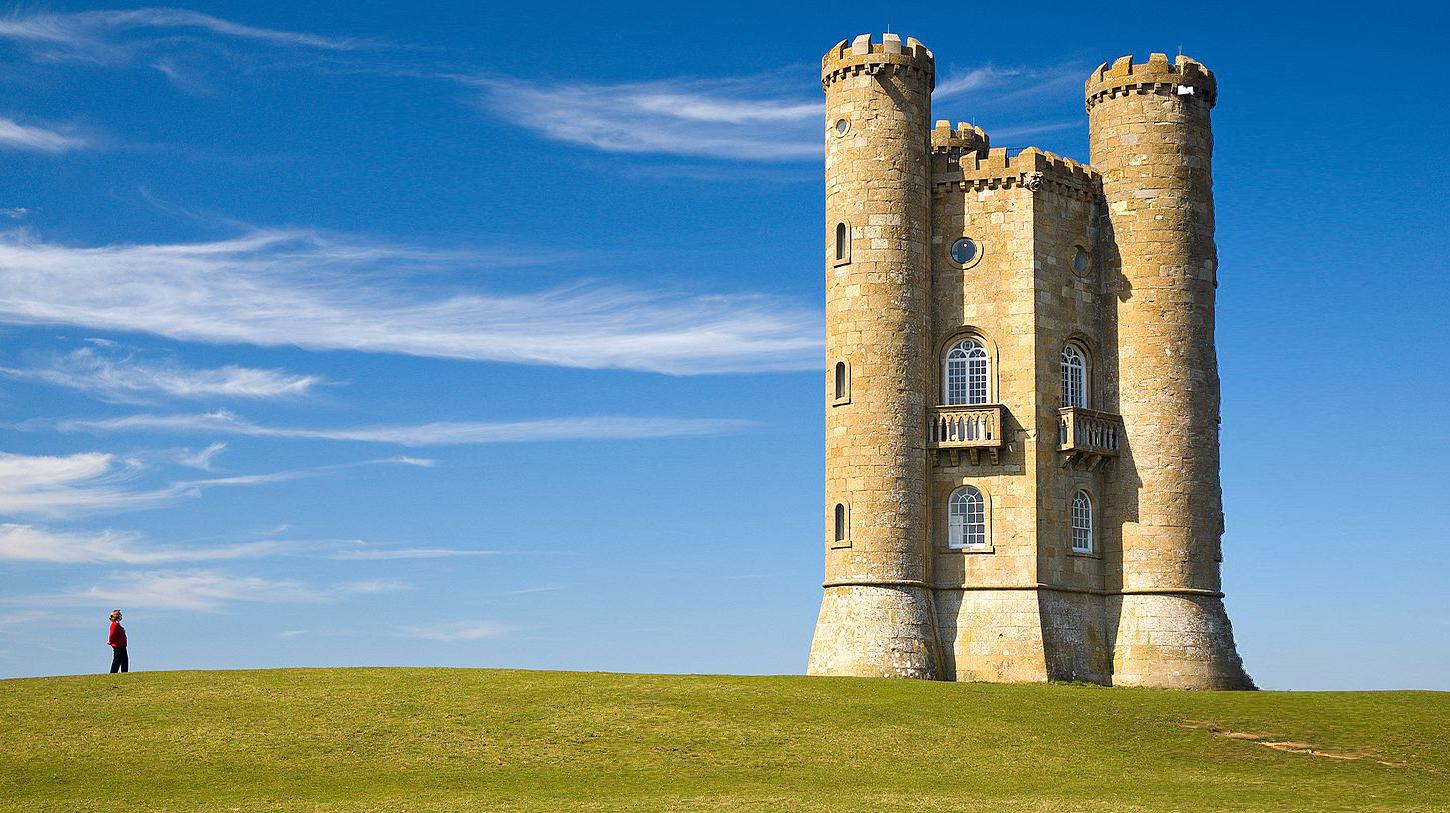
\includegraphics[width=\linewidth]{250-enlargementv.jpg}
      \caption{Resultado de ampliación por seam-carving con 250 hilos}\label{kinkakujiseam}
    \endminipage
\end{figure}

\section{Referencias}
\begin{enumerate}
\item Wikipedia contributors. "Seam carving." Wikipedia, The Free Encyclopedia.
 Wikipedia, The Free Encyclopedia, 14 Nov. 2018. Web. 15 Dec. 2018.
\item Wikipedia contributors. "Kernel (image processing)." Wikipedia, The Free Encyclopedia.
 Wikipedia, The Free Encyclopedia, 13 Dec. 2018. Web. 15 Dec. 2018. 
\item Wikipedia contributors. "Sobel operator." Wikipedia, The Free Encyclopedia.
 Wikipedia, The Free Encyclopedia, 27 Nov. 2018. Web. 15 Dec. 2018. 
\item Wikipedia contributors. "Kernel (image processing)." Wikipedia, The Free Encyclopedia.
 Wikipedia, The Free Encyclopedia, 13 Dec. 2018. Web. 15 Dec. 2018. 
\item Avidan, Shai, and Ariel Shamir. "Seam carving for content-aware image resizing."
 ACM Transactions on graphics (TOG). Vol. 26. No. 3. ACM, 2007.
\end{enumerate}
\end{document}

